\documentclass[twoside]{book}

% Packages required by doxygen
\usepackage{fixltx2e}
\usepackage{calc}
\usepackage{doxygen}
\usepackage[export]{adjustbox} % also loads graphicx
\usepackage{graphicx}
\usepackage[utf8]{inputenc}
\usepackage{makeidx}
\usepackage{multicol}
\usepackage{multirow}
\PassOptionsToPackage{warn}{textcomp}
\usepackage{textcomp}
\usepackage[nointegrals]{wasysym}
\usepackage[table]{xcolor}

% NLS support packages
\usepackage[french]{babel}
\NoAutoSpaceBeforeFDP

% Font selection
\usepackage[T1]{fontenc}
\usepackage[scaled=.90]{helvet}
\usepackage{courier}
\usepackage{amssymb}
\usepackage{sectsty}
\renewcommand{\familydefault}{\sfdefault}
\allsectionsfont{%
  \fontseries{bc}\selectfont%
  \color{darkgray}%
}
\renewcommand{\DoxyLabelFont}{%
  \fontseries{bc}\selectfont%
  \color{darkgray}%
}
\newcommand{\+}{\discretionary{\mbox{\scriptsize$\hookleftarrow$}}{}{}}

% Page & text layout
\usepackage{geometry}
\geometry{%
  a4paper,%
  top=2.5cm,%
  bottom=2.5cm,%
  left=2.5cm,%
  right=2.5cm%
}
\tolerance=750
\hfuzz=15pt
\hbadness=750
\setlength{\emergencystretch}{15pt}
\setlength{\parindent}{0cm}
\setlength{\parskip}{3ex plus 2ex minus 2ex}
\makeatletter
\renewcommand{\paragraph}{%
  \@startsection{paragraph}{4}{0ex}{-1.0ex}{1.0ex}{%
    \normalfont\normalsize\bfseries\SS@parafont%
  }%
}
\renewcommand{\subparagraph}{%
  \@startsection{subparagraph}{5}{0ex}{-1.0ex}{1.0ex}{%
    \normalfont\normalsize\bfseries\SS@subparafont%
  }%
}
\makeatother

% Headers & footers
\usepackage{fancyhdr}
\pagestyle{fancyplain}
\fancyhead[LE]{\fancyplain{}{\bfseries\thepage}}
\fancyhead[CE]{\fancyplain{}{}}
\fancyhead[RE]{\fancyplain{}{\bfseries\leftmark}}
\fancyhead[LO]{\fancyplain{}{\bfseries\rightmark}}
\fancyhead[CO]{\fancyplain{}{}}
\fancyhead[RO]{\fancyplain{}{\bfseries\thepage}}
\fancyfoot[LE]{\fancyplain{}{}}
\fancyfoot[CE]{\fancyplain{}{}}
\fancyfoot[RE]{\fancyplain{}{\bfseries\scriptsize Généré par Doxygen }}
\fancyfoot[LO]{\fancyplain{}{\bfseries\scriptsize Généré par Doxygen }}
\fancyfoot[CO]{\fancyplain{}{}}
\fancyfoot[RO]{\fancyplain{}{}}
\renewcommand{\footrulewidth}{0.4pt}
\renewcommand{\chaptermark}[1]{%
  \markboth{#1}{}%
}
\renewcommand{\sectionmark}[1]{%
  \markright{\thesection\ #1}%
}

% Indices & bibliography
\usepackage{natbib}
\usepackage[titles]{tocloft}
\setcounter{tocdepth}{3}
\setcounter{secnumdepth}{5}
\makeindex

% Hyperlinks (required, but should be loaded last)
\usepackage{ifpdf}
\ifpdf
  \usepackage[pdftex,pagebackref=true]{hyperref}
\else
  \usepackage[ps2pdf,pagebackref=true]{hyperref}
\fi
\hypersetup{%
  colorlinks=true,%
  linkcolor=blue,%
  citecolor=blue,%
  unicode%
}

% Custom commands
\newcommand{\clearemptydoublepage}{%
  \newpage{\pagestyle{empty}\cleardoublepage}%
}

\usepackage{caption}
\captionsetup{labelsep=space,justification=centering,font={bf},singlelinecheck=off,skip=4pt,position=top}

%===== C O N T E N T S =====

\begin{document}

% Titlepage & ToC
\hypersetup{pageanchor=false,
             bookmarksnumbered=true,
             pdfencoding=unicode
            }
\pagenumbering{alph}
\begin{titlepage}
\vspace*{7cm}
\begin{center}%
{\Large Logic\+Gate \\[1ex]\large 0.\+1 }\\
\vspace*{1cm}
{\large Généré par Doxygen 1.8.14}\\
\end{center}
\end{titlepage}
\clearemptydoublepage
\pagenumbering{roman}
\tableofcontents
\clearemptydoublepage
\pagenumbering{arabic}
\hypersetup{pageanchor=true}

%--- Begin generated contents ---
\chapter{Index hiérarchique}
\section{Hiérarchie des classes}
Cette liste d\textquotesingle{}héritage est classée approximativement par ordre alphabétique \+:\begin{DoxyCompactList}
\item \contentsline{section}{Anchor\+State}{\pageref{class_anchor_state}}{}
\item Mono\+Behaviour\begin{DoxyCompactList}
\item \contentsline{section}{Color\+Changer}{\pageref{class_color_changer}}{}
\item \contentsline{section}{Dont\+Destroy\+Param}{\pageref{class_dont_destroy_param}}{}
\item \contentsline{section}{Dont\+Destroy\+Speaker}{\pageref{class_dont_destroy_speaker}}{}
\item \contentsline{section}{Door}{\pageref{class_door}}{}
\item \contentsline{section}{Dragger}{\pageref{class_dragger}}{}
\begin{DoxyCompactList}
\item \contentsline{section}{Dragger\+Instantiater}{\pageref{class_dragger_instantiater}}{}
\end{DoxyCompactList}
\item \contentsline{section}{fils}{\pageref{classfils}}{}
\item \contentsline{section}{Grid\+Creater}{\pageref{class_grid_creater}}{}
\item \contentsline{section}{Load\+Scene}{\pageref{class_load_scene}}{}
\item \contentsline{section}{Load\+Scene\+Add}{\pageref{class_load_scene_add}}{}
\item \contentsline{section}{Parameters\+Loader}{\pageref{class_parameters_loader}}{}
\item \contentsline{section}{Pop\+Up\+Close}{\pageref{class_pop_up_close}}{}
\item \contentsline{section}{Quitter}{\pageref{class_quitter}}{}
\item \contentsline{section}{Remove\+Scene}{\pageref{class_remove_scene}}{}
\item \contentsline{section}{Save\+Param}{\pageref{class_save_param}}{}
\item \contentsline{section}{Snooze\+Changer}{\pageref{class_snooze_changer}}{}
\item \contentsline{section}{Volume\+Changer}{\pageref{class_volume_changer}}{}
\item \contentsline{section}{Volume\+Manager}{\pageref{class_volume_manager}}{}
\end{DoxyCompactList}
\item \contentsline{section}{Parameters}{\pageref{class_parameters}}{}
\end{DoxyCompactList}

\chapter{Index des classes}
\section{Liste des classes}
Liste des classes, structures, unions et interfaces avec une brève description \+:\begin{DoxyCompactList}
\item\contentsline{section}{\mbox{\hyperlink{class_anchor_state}{Anchor\+State}} \\*C\textquotesingle{}est une ancre qui va posséder sa position ainsi que sa liberté }{\pageref{class_anchor_state}}{}
\item\contentsline{section}{\mbox{\hyperlink{class_color_changer}{Color\+Changer}} }{\pageref{class_color_changer}}{}
\item\contentsline{section}{\mbox{\hyperlink{class_dont_destroy_param}{Dont\+Destroy\+Param}} }{\pageref{class_dont_destroy_param}}{}
\item\contentsline{section}{\mbox{\hyperlink{class_dont_destroy_speaker}{Dont\+Destroy\+Speaker}} }{\pageref{class_dont_destroy_speaker}}{}
\item\contentsline{section}{\mbox{\hyperlink{class_door}{Door}} }{\pageref{class_door}}{}
\item\contentsline{section}{\mbox{\hyperlink{class_dragger}{Dragger}} }{\pageref{class_dragger}}{}
\item\contentsline{section}{\mbox{\hyperlink{class_dragger_instantiater}{Dragger\+Instantiater}} }{\pageref{class_dragger_instantiater}}{}
\item\contentsline{section}{\mbox{\hyperlink{classfils}{fils}} }{\pageref{classfils}}{}
\item\contentsline{section}{\mbox{\hyperlink{class_grid_creater}{Grid\+Creater}} \\*Création de la grille de jeu }{\pageref{class_grid_creater}}{}
\item\contentsline{section}{\mbox{\hyperlink{class_load_scene}{Load\+Scene}} }{\pageref{class_load_scene}}{}
\item\contentsline{section}{\mbox{\hyperlink{class_load_scene_add}{Load\+Scene\+Add}} }{\pageref{class_load_scene_add}}{}
\item\contentsline{section}{\mbox{\hyperlink{class_parameters}{Parameters}} }{\pageref{class_parameters}}{}
\item\contentsline{section}{\mbox{\hyperlink{class_parameters_loader}{Parameters\+Loader}} }{\pageref{class_parameters_loader}}{}
\item\contentsline{section}{\mbox{\hyperlink{class_pop_up_close}{Pop\+Up\+Close}} }{\pageref{class_pop_up_close}}{}
\item\contentsline{section}{\mbox{\hyperlink{class_quitter}{Quitter}} }{\pageref{class_quitter}}{}
\item\contentsline{section}{\mbox{\hyperlink{class_remove_scene}{Remove\+Scene}} }{\pageref{class_remove_scene}}{}
\item\contentsline{section}{\mbox{\hyperlink{class_save_param}{Save\+Param}} }{\pageref{class_save_param}}{}
\item\contentsline{section}{\mbox{\hyperlink{class_snooze_changer}{Snooze\+Changer}} }{\pageref{class_snooze_changer}}{}
\item\contentsline{section}{\mbox{\hyperlink{class_volume_changer}{Volume\+Changer}} }{\pageref{class_volume_changer}}{}
\item\contentsline{section}{\mbox{\hyperlink{class_volume_manager}{Volume\+Manager}} }{\pageref{class_volume_manager}}{}
\end{DoxyCompactList}

\chapter{Documentation des classes}
\hypertarget{class_anchor_state}{}\section{Référence de la classe Anchor\+State}
\label{class_anchor_state}\index{Anchor\+State@{Anchor\+State}}


C\textquotesingle{}est une ancre qui va posséder sa position ainsi que sa liberté  


\subsection*{Fonctions membres publiques}
\begin{DoxyCompactItemize}
\item 
\mbox{\Hypertarget{class_anchor_state_a6f09a84b1fa65d14f5757ec975aa9bf3}\label{class_anchor_state_a6f09a84b1fa65d14f5757ec975aa9bf3}} 
{\bfseries Anchor\+State} (Vector3 \mbox{\hyperlink{class_anchor_state_aedc18ef657d28aec45ad3fd88e485123}{position}})
\end{DoxyCompactItemize}
\subsection*{Attributs publics}
\begin{DoxyCompactItemize}
\item 
\mbox{\Hypertarget{class_anchor_state_af84faa58def0c07ce1deae74bf137b94}\label{class_anchor_state_af84faa58def0c07ce1deae74bf137b94}} 
bool \mbox{\hyperlink{class_anchor_state_af84faa58def0c07ce1deae74bf137b94}{free}}
\begin{DoxyCompactList}\small\item\em Definie la liberté de l\textquotesingle{}ancre. \end{DoxyCompactList}\item 
\mbox{\Hypertarget{class_anchor_state_aedc18ef657d28aec45ad3fd88e485123}\label{class_anchor_state_aedc18ef657d28aec45ad3fd88e485123}} 
Vector3 \mbox{\hyperlink{class_anchor_state_aedc18ef657d28aec45ad3fd88e485123}{position}}
\begin{DoxyCompactList}\small\item\em Position de l\textquotesingle{}ancre. \end{DoxyCompactList}\end{DoxyCompactItemize}


\subsection{Description détaillée}
C\textquotesingle{}est une ancre qui va posséder sa position ainsi que sa liberté 

La documentation de cette classe a été générée à partir du fichier suivant \+:\begin{DoxyCompactItemize}
\item 
F\+:/\+Logic\+Gate/\+Logic\+Gate3/\+Unity\+Project/\+Assets/\+Our\+Scripts/Grid\+Creater.\+cs\end{DoxyCompactItemize}

\hypertarget{class_color_changer}{}\section{Référence de la classe Color\+Changer}
\label{class_color_changer}\index{Color\+Changer@{Color\+Changer}}
Graphe d\textquotesingle{}héritage de Color\+Changer\+:\begin{figure}[H]
\begin{center}
\leavevmode
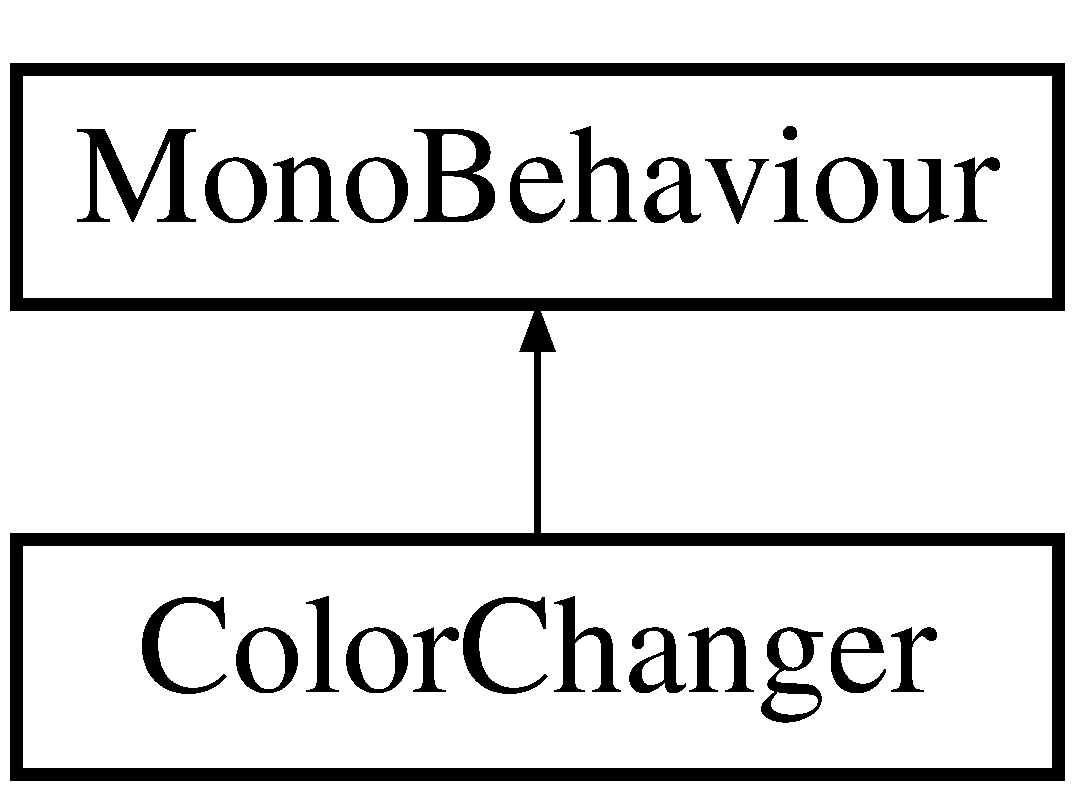
\includegraphics[height=2.000000cm]{class_color_changer}
\end{center}
\end{figure}
\subsection*{Attributs publics}
\begin{DoxyCompactItemize}
\item 
\mbox{\Hypertarget{class_color_changer_a0a73a532b8ee1f26dbc3b8944f33b6e4}\label{class_color_changer_a0a73a532b8ee1f26dbc3b8944f33b6e4}} 
\mbox{\hyperlink{class_parameters}{Parameters}} {\bfseries manager}
\end{DoxyCompactItemize}


La documentation de cette classe a été générée à partir du fichier suivant \+:\begin{DoxyCompactItemize}
\item 
F\+:/\+Logic\+Gate/\+Logic\+Gate3/\+Unity\+Project/\+Assets/\+Our\+Scripts/Color\+Changer.\+cs\end{DoxyCompactItemize}

\hypertarget{class_dont_destroy_param}{}\section{Référence de la classe Dont\+Destroy\+Param}
\label{class_dont_destroy_param}\index{Dont\+Destroy\+Param@{Dont\+Destroy\+Param}}
Graphe d\textquotesingle{}héritage de Dont\+Destroy\+Param\+:\begin{figure}[H]
\begin{center}
\leavevmode
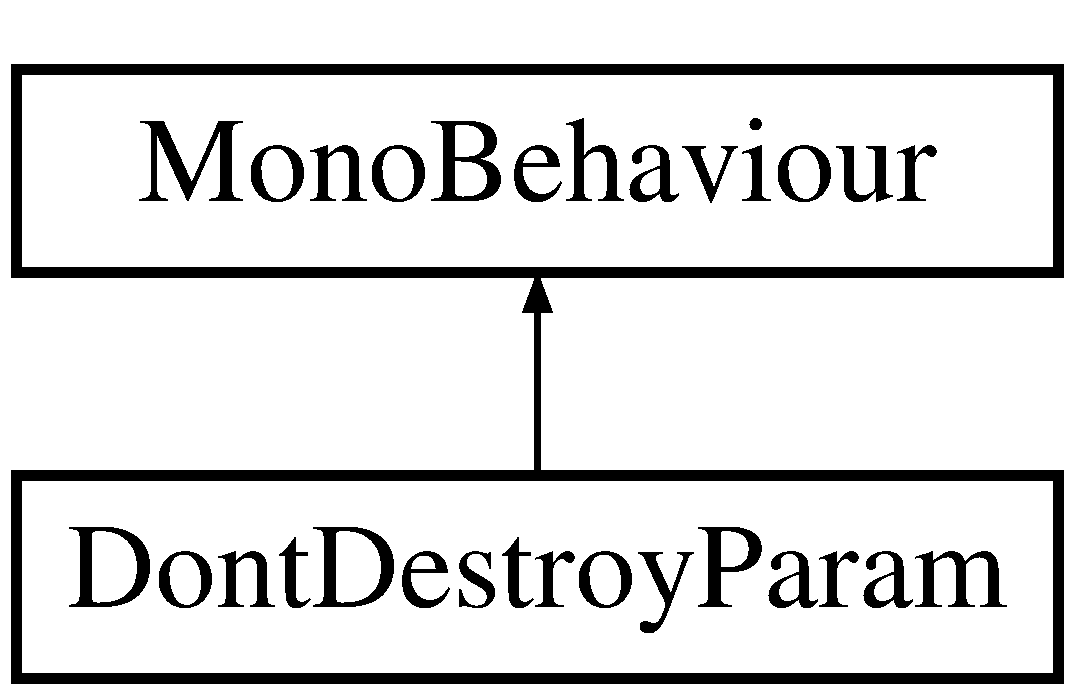
\includegraphics[height=2.000000cm]{class_dont_destroy_param}
\end{center}
\end{figure}


La documentation de cette classe a été générée à partir du fichier suivant \+:\begin{DoxyCompactItemize}
\item 
F\+:/\+Logic\+Gate/\+Logic\+Gate3/\+Unity\+Project/\+Assets/\+Our\+Scripts/Dont\+Destroy\+Param.\+cs\end{DoxyCompactItemize}

\hypertarget{class_dont_destroy_speaker}{}\section{Référence de la classe Dont\+Destroy\+Speaker}
\label{class_dont_destroy_speaker}\index{Dont\+Destroy\+Speaker@{Dont\+Destroy\+Speaker}}
Graphe d\textquotesingle{}héritage de Dont\+Destroy\+Speaker\+:\begin{figure}[H]
\begin{center}
\leavevmode
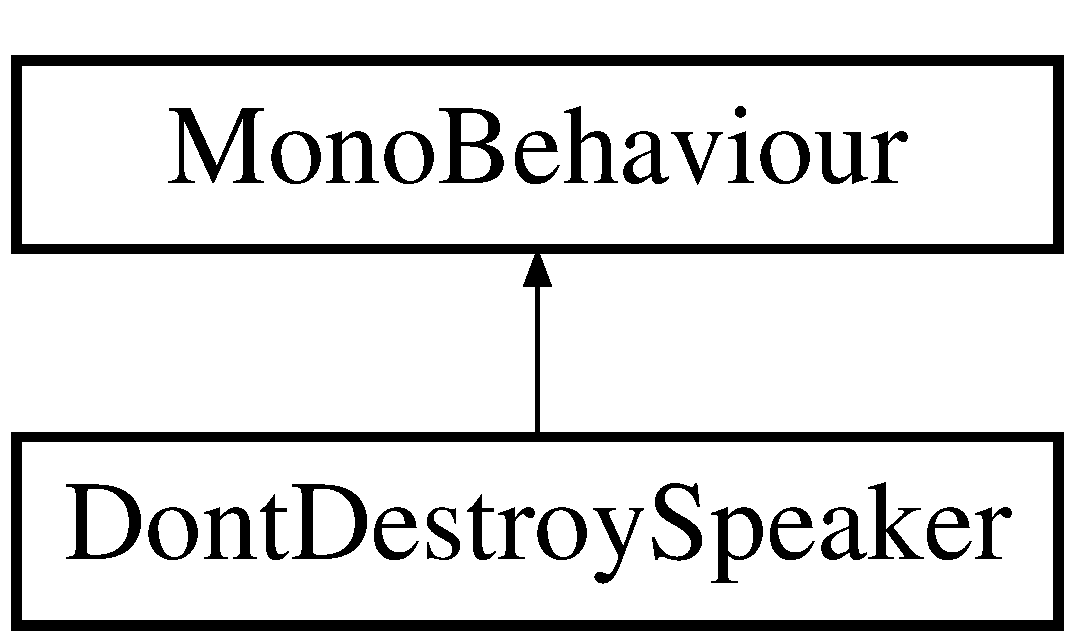
\includegraphics[height=2.000000cm]{class_dont_destroy_speaker}
\end{center}
\end{figure}


La documentation de cette classe a été générée à partir du fichier suivant \+:\begin{DoxyCompactItemize}
\item 
F\+:/\+Logic\+Gate/\+Logic\+Gate3/\+Unity\+Project/\+Assets/\+Our\+Scripts/Dont\+Destroy\+Speaker.\+cs\end{DoxyCompactItemize}

\hypertarget{class_door}{}\section{Référence de la classe Door}
\label{class_door}\index{Door@{Door}}
Graphe d\textquotesingle{}héritage de Door\+:\begin{figure}[H]
\begin{center}
\leavevmode
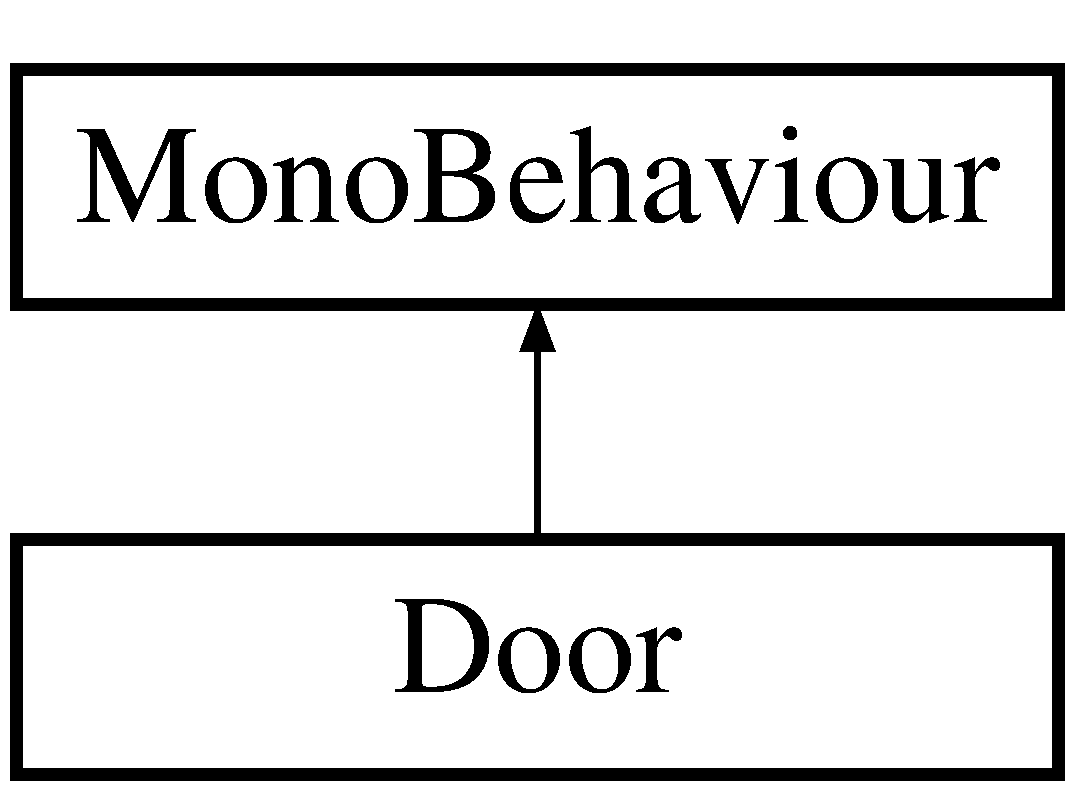
\includegraphics[height=2.000000cm]{class_door}
\end{center}
\end{figure}
\subsection*{Fonctions membres publiques}
\begin{DoxyCompactItemize}
\item 
\mbox{\Hypertarget{class_door_a4f710644553e0909584c57d2eac9a69b}\label{class_door_a4f710644553e0909584c57d2eac9a69b}} 
\mbox{\hyperlink{class_door}{Door}} {\bfseries Linked\+To} ()
\end{DoxyCompactItemize}
\subsection*{Attributs publics}
\begin{DoxyCompactItemize}
\item 
\mbox{\Hypertarget{class_door_af18a6dccacf615f278ab503e25cafeb9}\label{class_door_af18a6dccacf615f278ab503e25cafeb9}} 
bool {\bfseries power} = false
\end{DoxyCompactItemize}


La documentation de cette classe a été générée à partir du fichier suivant \+:\begin{DoxyCompactItemize}
\item 
F\+:/\+Logic\+Gate/\+Logic\+Gate3/\+Unity\+Project/\+Assets/\+Our\+Scripts/Door.\+cs\end{DoxyCompactItemize}

\hypertarget{class_dragger}{}\section{Référence de la classe Dragger}
\label{class_dragger}\index{Dragger@{Dragger}}
Graphe d\textquotesingle{}héritage de Dragger\+:\begin{figure}[H]
\begin{center}
\leavevmode
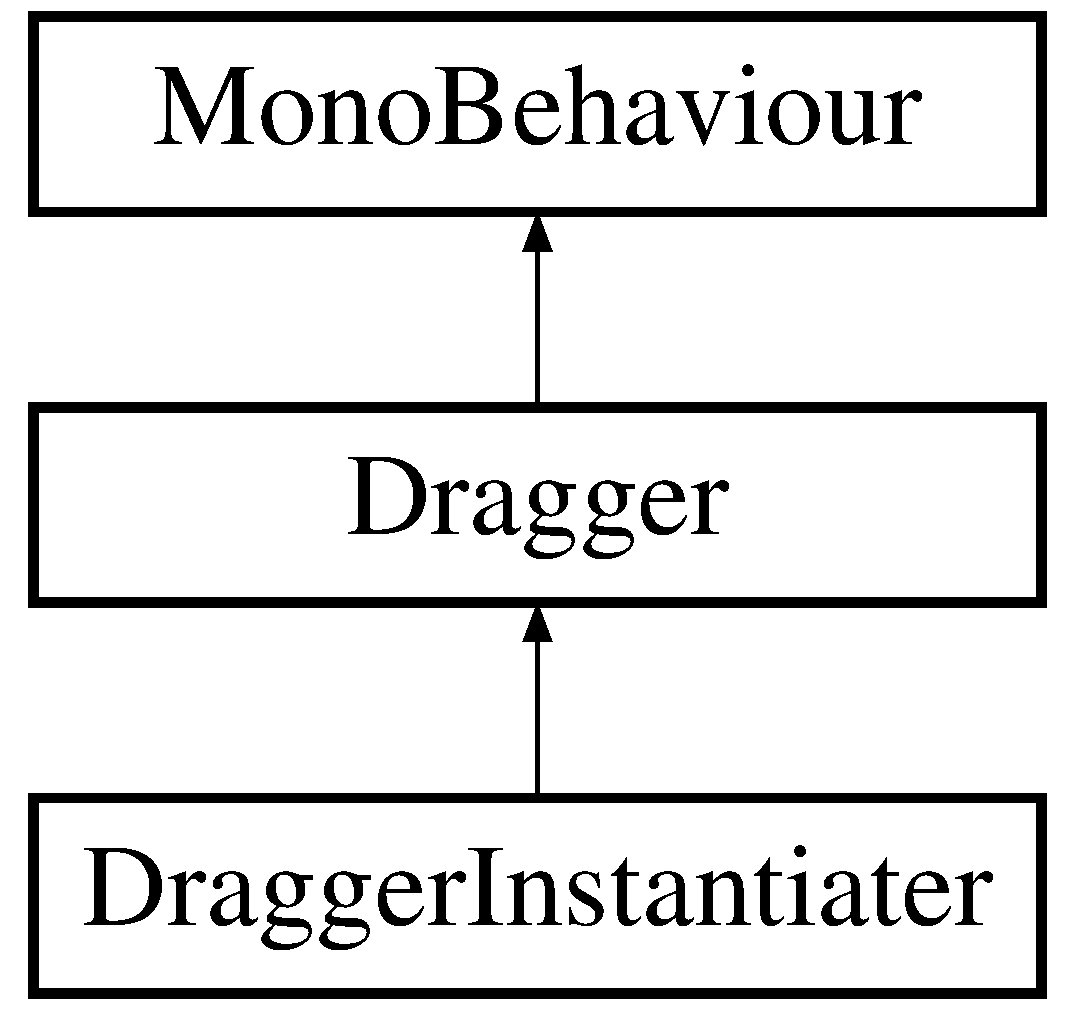
\includegraphics[height=3.000000cm]{class_dragger}
\end{center}
\end{figure}
\subsection*{Fonctions membres publiques}
\begin{DoxyCompactItemize}
\item 
\mbox{\Hypertarget{class_dragger_a5ff1ad4684c5f1f6fb0c6eb66386c321}\label{class_dragger_a5ff1ad4684c5f1f6fb0c6eb66386c321}} 
\mbox{\hyperlink{class_anchor_state}{Anchor\+State}} \mbox{\hyperlink{class_dragger_a5ff1ad4684c5f1f6fb0c6eb66386c321}{Find\+Nearest}} (List$<$ \mbox{\hyperlink{class_anchor_state}{Anchor\+State}} $>$ anchor\+\_\+list, Game\+Object to\+\_\+move)
\begin{DoxyCompactList}\small\item\em Find the nearest anchor in the list form the given object. \end{DoxyCompactList}\item 
\mbox{\Hypertarget{class_dragger_ac88471862f06150a27622527978fc672}\label{class_dragger_ac88471862f06150a27622527978fc672}} 
void {\bfseries Destroy\+On\+Bin} (Game\+Object obj)
\item 
void \mbox{\hyperlink{class_dragger_a0c35e5fa5a41f5f0ba823ecc94d94801}{On\+Mouse\+Down}} ()
\item 
void \mbox{\hyperlink{class_dragger_a6fefaac4e505d917405736eafa051463}{On\+Mouse\+Up}} ()
\item 
\mbox{\Hypertarget{class_dragger_ad992b4962d200f6a323b4abf93206a6f}\label{class_dragger_ad992b4962d200f6a323b4abf93206a6f}} 
void \mbox{\hyperlink{class_dragger_ad992b4962d200f6a323b4abf93206a6f}{Update}} ()
\begin{DoxyCompactList}\small\item\em if the mouse is pressed the object follow the mouse pointer \end{DoxyCompactList}\end{DoxyCompactItemize}
\subsection*{Attributs publics}
\begin{DoxyCompactItemize}
\item 
\mbox{\Hypertarget{class_dragger_a1d16edf9f508d52493bda6130d9188d7}\label{class_dragger_a1d16edf9f508d52493bda6130d9188d7}} 
Vector3 {\bfseries initial\+Obj\+Mouse\+Distance}
\item 
\mbox{\Hypertarget{class_dragger_a916c768cb219dee4d24ab41d869f1b4b}\label{class_dragger_a916c768cb219dee4d24ab41d869f1b4b}} 
bool {\bfseries mouse\+Down} = false
\item 
\mbox{\Hypertarget{class_dragger_ae6877a2d7c8622dbebad040d764cc70e}\label{class_dragger_ae6877a2d7c8622dbebad040d764cc70e}} 
\mbox{\hyperlink{class_anchor_state}{Anchor\+State}} {\bfseries anchor\+Point} = null
\end{DoxyCompactItemize}


\subsection{Documentation des fonctions membres}
\mbox{\Hypertarget{class_dragger_a0c35e5fa5a41f5f0ba823ecc94d94801}\label{class_dragger_a0c35e5fa5a41f5f0ba823ecc94d94801}} 
\index{Dragger@{Dragger}!On\+Mouse\+Down@{On\+Mouse\+Down}}
\index{On\+Mouse\+Down@{On\+Mouse\+Down}!Dragger@{Dragger}}
\subsubsection{\texorpdfstring{On\+Mouse\+Down()}{OnMouseDown()}}
{\footnotesize\ttfamily void Dragger.\+On\+Mouse\+Down (\begin{DoxyParamCaption}{ }\end{DoxyParamCaption})}

To avoid the object going right under the mouse cursor \mbox{\Hypertarget{class_dragger_a6fefaac4e505d917405736eafa051463}\label{class_dragger_a6fefaac4e505d917405736eafa051463}} 
\index{Dragger@{Dragger}!On\+Mouse\+Up@{On\+Mouse\+Up}}
\index{On\+Mouse\+Up@{On\+Mouse\+Up}!Dragger@{Dragger}}
\subsubsection{\texorpdfstring{On\+Mouse\+Up()}{OnMouseUp()}}
{\footnotesize\ttfamily void Dragger.\+On\+Mouse\+Up (\begin{DoxyParamCaption}{ }\end{DoxyParamCaption})}

Place the object on the nearest anchor 

La documentation de cette classe a été générée à partir du fichier suivant \+:\begin{DoxyCompactItemize}
\item 
F\+:/\+Logic\+Gate/\+Logic\+Gate3/\+Unity\+Project/\+Assets/\+Our\+Scripts/\+Dragging/Dragger.\+cs\end{DoxyCompactItemize}

\hypertarget{class_dragger_instantiater}{}\section{Référence de la classe Dragger\+Instantiater}
\label{class_dragger_instantiater}\index{Dragger\+Instantiater@{Dragger\+Instantiater}}
Graphe d\textquotesingle{}héritage de Dragger\+Instantiater\+:\begin{figure}[H]
\begin{center}
\leavevmode
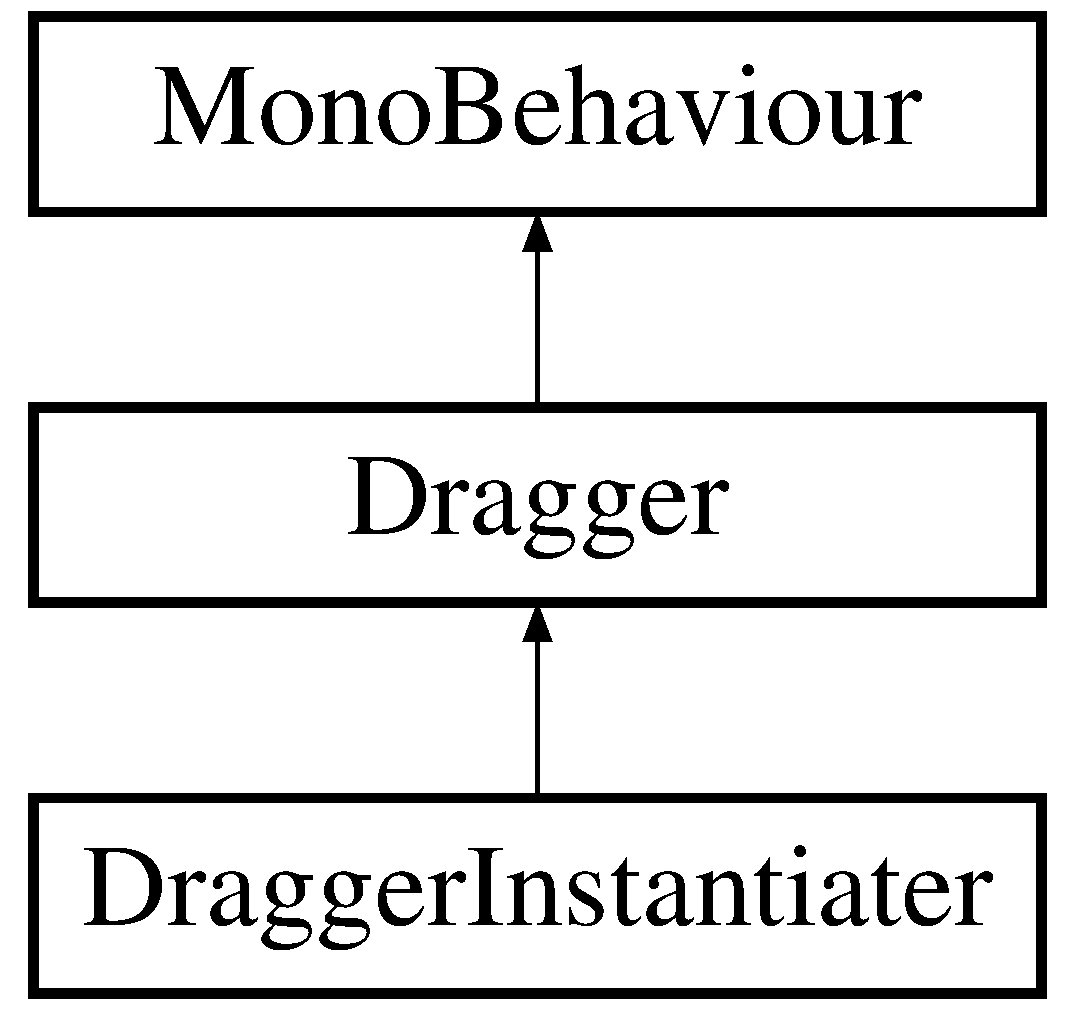
\includegraphics[height=3.000000cm]{class_dragger_instantiater}
\end{center}
\end{figure}
\subsection*{Membres hérités additionnels}


La documentation de cette classe a été générée à partir du fichier suivant \+:\begin{DoxyCompactItemize}
\item 
F\+:/\+Logic\+Gate/\+Logic\+Gate3/\+Unity\+Project/\+Assets/\+Our\+Scripts/\+Dragging/Dragger\+Instantiater.\+cs\end{DoxyCompactItemize}

\hypertarget{classfils}{}\section{Référence de la classe fils}
\label{classfils}\index{fils@{fils}}
Graphe d\textquotesingle{}héritage de fils\+:\begin{figure}[H]
\begin{center}
\leavevmode
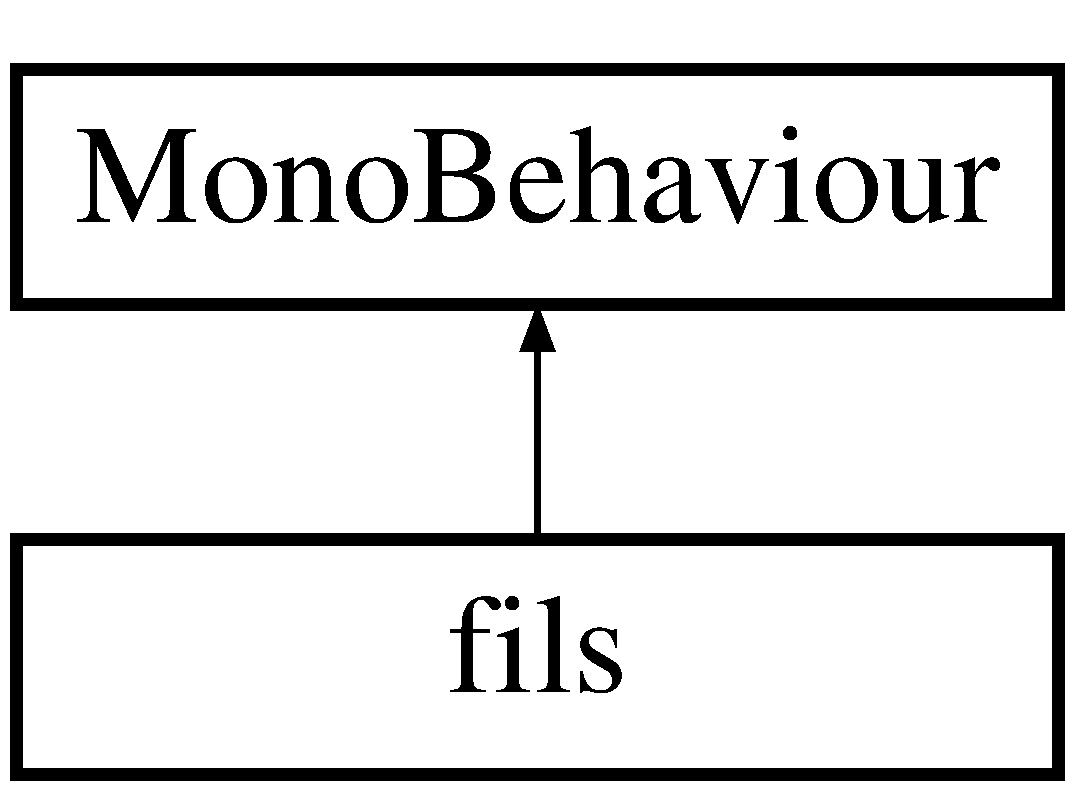
\includegraphics[height=2.000000cm]{classfils}
\end{center}
\end{figure}
\subsection*{Attributs publics}
\begin{DoxyCompactItemize}
\item 
\mbox{\Hypertarget{classfils_a75fa93b25ebb43aa75d18ec676f5ec38}\label{classfils_a75fa93b25ebb43aa75d18ec676f5ec38}} 
bool {\bfseries powered} = false
\end{DoxyCompactItemize}


La documentation de cette classe a été générée à partir du fichier suivant \+:\begin{DoxyCompactItemize}
\item 
F\+:/\+Logic\+Gate/\+Logic\+Gate3/\+Unity\+Project/\+Assets/\+Our\+Scripts/fils.\+cs\end{DoxyCompactItemize}

\hypertarget{class_grid_creater}{}\section{Référence de la classe Grid\+Creater}
\label{class_grid_creater}\index{Grid\+Creater@{Grid\+Creater}}


Création de la grille de jeu.  


Graphe d\textquotesingle{}héritage de Grid\+Creater\+:\begin{figure}[H]
\begin{center}
\leavevmode
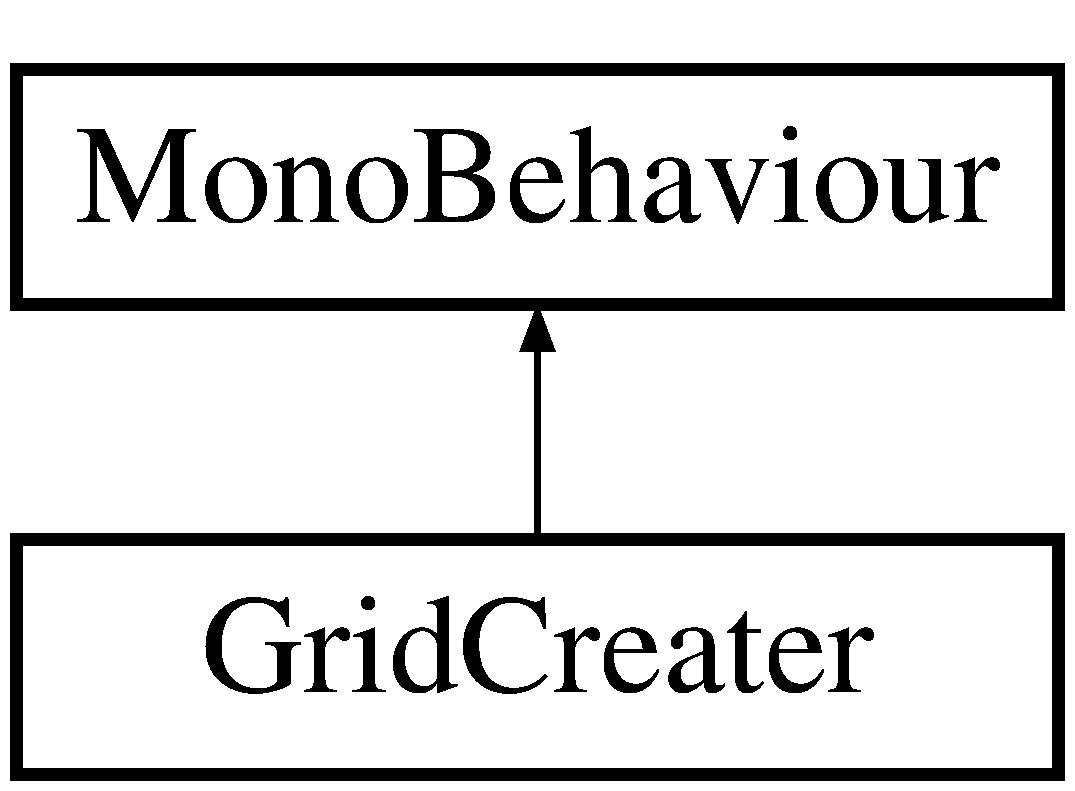
\includegraphics[height=2.000000cm]{class_grid_creater}
\end{center}
\end{figure}
\subsection*{Attributs publics}
\begin{DoxyCompactItemize}
\item 
\mbox{\Hypertarget{class_grid_creater_a2e6b4a0cbfd8941b319385ad0b62b2b5}\label{class_grid_creater_a2e6b4a0cbfd8941b319385ad0b62b2b5}} 
int {\bfseries grid\+\_\+divisions} = 10
\item 
\mbox{\Hypertarget{class_grid_creater_ade7062c5dca408381c99fd7ffe97428c}\label{class_grid_creater_ade7062c5dca408381c99fd7ffe97428c}} 
Material {\bfseries material}
\item 
\mbox{\Hypertarget{class_grid_creater_ae889352fee8745fdea823238abc580c6}\label{class_grid_creater_ae889352fee8745fdea823238abc580c6}} 
List$<$ \mbox{\hyperlink{class_anchor_state}{Anchor\+State}} $>$ \mbox{\hyperlink{class_grid_creater_ae889352fee8745fdea823238abc580c6}{anchor\+\_\+list}} = new List$<$\mbox{\hyperlink{class_anchor_state}{Anchor\+State}}$>$()
\begin{DoxyCompactList}\small\item\em Liste des ancres auquel on pourra accrocher les portes. \end{DoxyCompactList}\end{DoxyCompactItemize}
\textbf{ }\par
\begin{DoxyCompactItemize}
\item 
int \mbox{\hyperlink{class_grid_creater_a1b96eaac4e4622871415c70ee7933ee9}{x\+Left}}
\item 
\mbox{\Hypertarget{class_grid_creater_acd450558c47b141e6ca647c577afc01b}\label{class_grid_creater_acd450558c47b141e6ca647c577afc01b}} 
int {\bfseries x\+Right}
\item 
\mbox{\Hypertarget{class_grid_creater_ab6ccca1c9c4ac6afaa5e294f0795ef55}\label{class_grid_creater_ab6ccca1c9c4ac6afaa5e294f0795ef55}} 
int {\bfseries y\+Bottom}
\item 
\mbox{\Hypertarget{class_grid_creater_a982daa5a2b4ee0afff04ca99328a30f2}\label{class_grid_creater_a982daa5a2b4ee0afff04ca99328a30f2}} 
int {\bfseries y\+Top}
\end{DoxyCompactItemize}



\subsection{Description détaillée}
Création de la grille de jeu. 

\subsection{Documentation des données membres}
\mbox{\Hypertarget{class_grid_creater_a1b96eaac4e4622871415c70ee7933ee9}\label{class_grid_creater_a1b96eaac4e4622871415c70ee7933ee9}} 
\index{Grid\+Creater@{Grid\+Creater}!x\+Left@{x\+Left}}
\index{x\+Left@{x\+Left}!Grid\+Creater@{Grid\+Creater}}
\subsubsection{\texorpdfstring{x\+Left}{xLeft}}
{\footnotesize\ttfamily int Grid\+Creater.\+x\+Left}

Position des différent points de référence de la grille 

La documentation de cette classe a été générée à partir du fichier suivant \+:\begin{DoxyCompactItemize}
\item 
F\+:/\+Logic\+Gate/\+Logic\+Gate3/\+Unity\+Project/\+Assets/\+Our\+Scripts/Grid\+Creater.\+cs\end{DoxyCompactItemize}

\hypertarget{class_load_scene}{}\section{Référence de la classe Load\+Scene}
\label{class_load_scene}\index{Load\+Scene@{Load\+Scene}}
Graphe d\textquotesingle{}héritage de Load\+Scene\+:\begin{figure}[H]
\begin{center}
\leavevmode
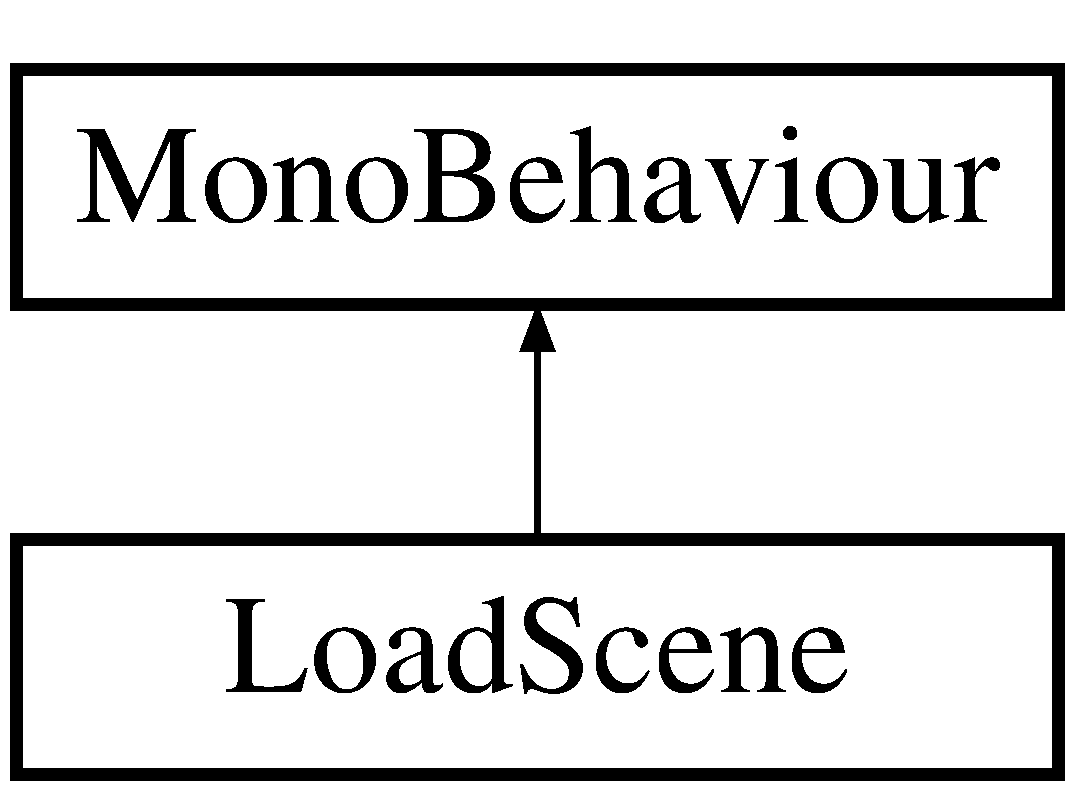
\includegraphics[height=2.000000cm]{class_load_scene}
\end{center}
\end{figure}
\subsection*{Fonctions membres publiques}
\begin{DoxyCompactItemize}
\item 
\mbox{\Hypertarget{class_load_scene_a14b31f2bd3ebd80e6561f17468892db3}\label{class_load_scene_a14b31f2bd3ebd80e6561f17468892db3}} 
void {\bfseries On\+Click} ()
\end{DoxyCompactItemize}
\subsection*{Attributs publics}
\begin{DoxyCompactItemize}
\item 
\mbox{\Hypertarget{class_load_scene_a5b9aeb8ede8c3f3e65243edad89d9c1e}\label{class_load_scene_a5b9aeb8ede8c3f3e65243edad89d9c1e}} 
string {\bfseries scene\+To\+Load}
\end{DoxyCompactItemize}


La documentation de cette classe a été générée à partir du fichier suivant \+:\begin{DoxyCompactItemize}
\item 
F\+:/\+Logic\+Gate/\+Logic\+Gate3/\+Unity\+Project/\+Assets/\+Our\+Scripts/Load\+Scene.\+cs\end{DoxyCompactItemize}

\hypertarget{class_load_scene_add}{}\section{Référence de la classe Load\+Scene\+Add}
\label{class_load_scene_add}\index{Load\+Scene\+Add@{Load\+Scene\+Add}}
Graphe d\textquotesingle{}héritage de Load\+Scene\+Add\+:\begin{figure}[H]
\begin{center}
\leavevmode
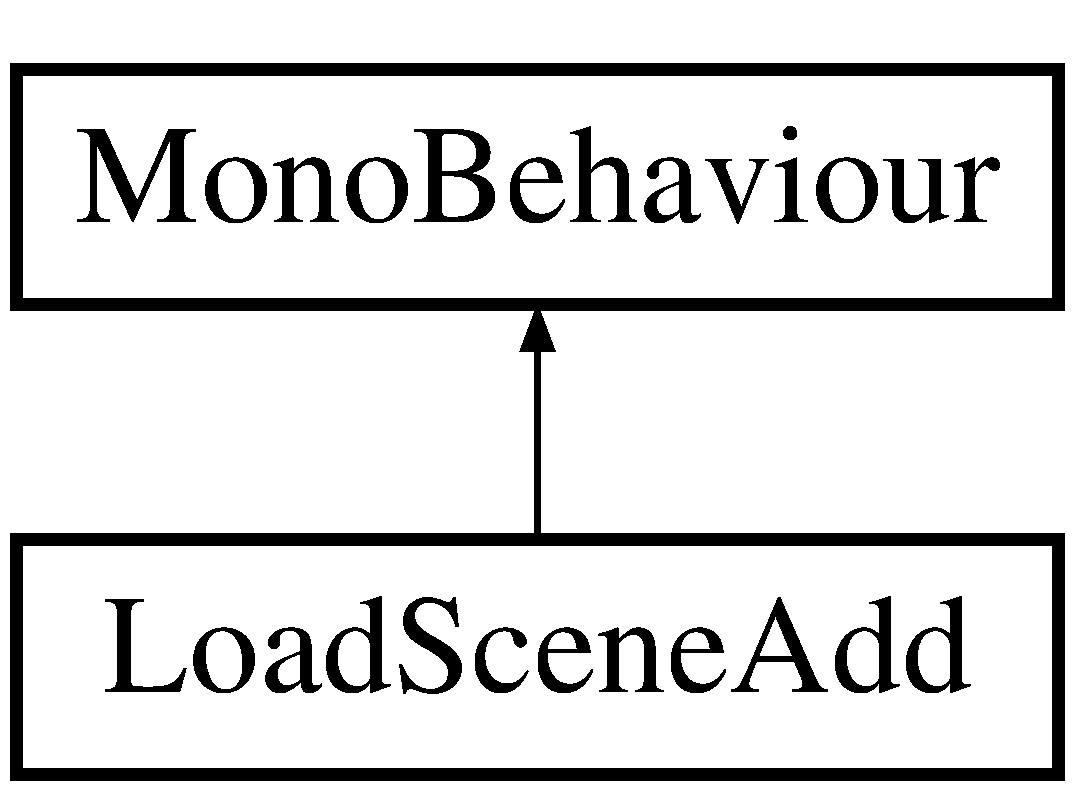
\includegraphics[height=2.000000cm]{class_load_scene_add}
\end{center}
\end{figure}
\subsection*{Fonctions membres publiques}
\begin{DoxyCompactItemize}
\item 
\mbox{\Hypertarget{class_load_scene_add_ab3265a9d67e26dbd627c339785eb8749}\label{class_load_scene_add_ab3265a9d67e26dbd627c339785eb8749}} 
void {\bfseries On\+Click} ()
\end{DoxyCompactItemize}
\subsection*{Attributs publics}
\begin{DoxyCompactItemize}
\item 
\mbox{\Hypertarget{class_load_scene_add_ae41b80a61d0923d997a6343e35355727}\label{class_load_scene_add_ae41b80a61d0923d997a6343e35355727}} 
string {\bfseries scene\+To\+Load}
\end{DoxyCompactItemize}


La documentation de cette classe a été générée à partir du fichier suivant \+:\begin{DoxyCompactItemize}
\item 
F\+:/\+Logic\+Gate/\+Logic\+Gate3/\+Unity\+Project/\+Assets/\+Our\+Scripts/Load\+Scene\+Add.\+cs\end{DoxyCompactItemize}

\hypertarget{class_parameters}{}\section{Référence de la classe Parameters}
\label{class_parameters}\index{Parameters@{Parameters}}
\subsection*{Fonctions membres publiques}
\begin{DoxyCompactItemize}
\item 
\mbox{\Hypertarget{class_parameters_adeed4b45e120cbbba31153e7c8e2dc9a}\label{class_parameters_adeed4b45e120cbbba31153e7c8e2dc9a}} 
void {\bfseries Load\+Parameters} ()
\item 
\mbox{\Hypertarget{class_parameters_a9651655951b8db0a4f7b6e3bee48e9ac}\label{class_parameters_a9651655951b8db0a4f7b6e3bee48e9ac}} 
void {\bfseries change\+\_\+snooze} ()
\end{DoxyCompactItemize}
\subsection*{Attributs publics}
\begin{DoxyCompactItemize}
\item 
\mbox{\Hypertarget{class_parameters_a59453e68e6a3d176b82264ec4098ce2d}\label{class_parameters_a59453e68e6a3d176b82264ec4098ce2d}} 
float {\bfseries music\+\_\+volume}
\item 
\mbox{\Hypertarget{class_parameters_aa9c08ea71b0805eee7571d21a857afa4}\label{class_parameters_aa9c08ea71b0805eee7571d21a857afa4}} 
bool {\bfseries snooze}
\item 
\mbox{\Hypertarget{class_parameters_a606a40250d5734587390ff228f97fefd}\label{class_parameters_a606a40250d5734587390ff228f97fefd}} 
float {\bfseries color}
\end{DoxyCompactItemize}


La documentation de cette classe a été générée à partir du fichier suivant \+:\begin{DoxyCompactItemize}
\item 
F\+:/\+Logic\+Gate/\+Logic\+Gate3/\+Unity\+Project/\+Assets/\+Our\+Scripts/Parameters.\+cs\end{DoxyCompactItemize}

\hypertarget{class_parameters_loader}{}\section{Référence de la classe Parameters\+Loader}
\label{class_parameters_loader}\index{Parameters\+Loader@{Parameters\+Loader}}
Graphe d\textquotesingle{}héritage de Parameters\+Loader\+:\begin{figure}[H]
\begin{center}
\leavevmode
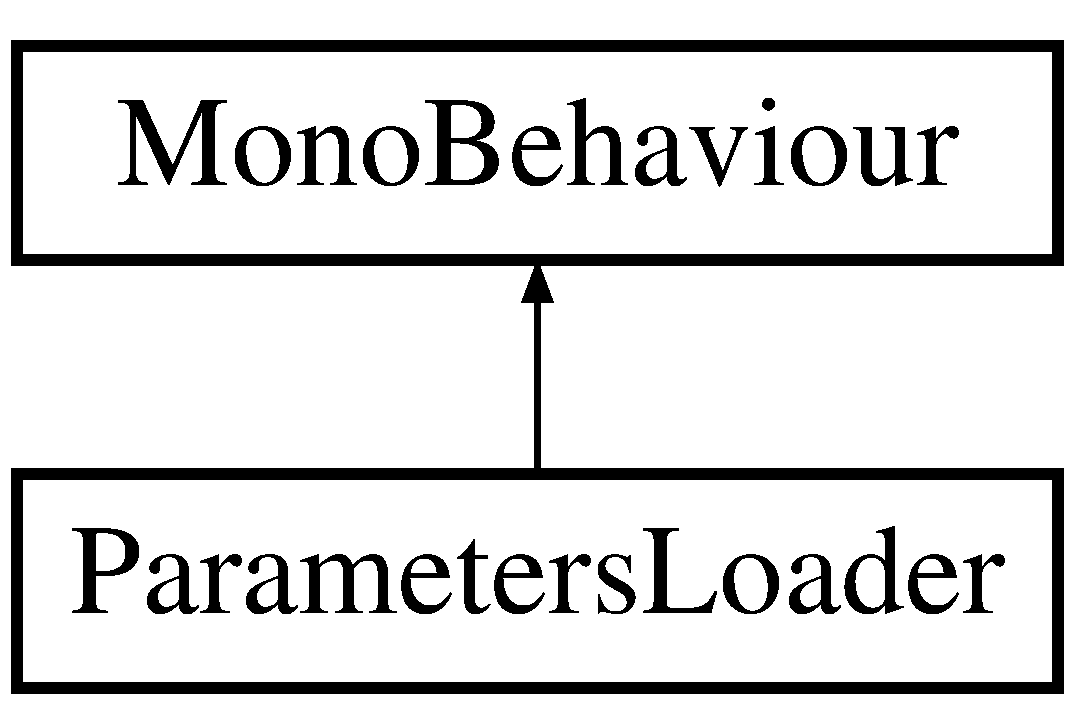
\includegraphics[height=2.000000cm]{class_parameters_loader}
\end{center}
\end{figure}
\subsection*{Fonctions membres publiques}
\begin{DoxyCompactItemize}
\item 
\mbox{\Hypertarget{class_parameters_loader_a7150dc98b0bf3c29d6f0c2494314ab1f}\label{class_parameters_loader_a7150dc98b0bf3c29d6f0c2494314ab1f}} 
void {\bfseries Start} ()
\end{DoxyCompactItemize}
\subsection*{Fonctions membres publiques statiques}
\begin{DoxyCompactItemize}
\item 
\mbox{\Hypertarget{class_parameters_loader_afeda242af9632639661957a7a46c8a1a}\label{class_parameters_loader_afeda242af9632639661957a7a46c8a1a}} 
static float {\bfseries Get\+Music\+Volume} ()
\item 
\mbox{\Hypertarget{class_parameters_loader_ad4e278bf9cc9a5aed98032241fb0c6b8}\label{class_parameters_loader_ad4e278bf9cc9a5aed98032241fb0c6b8}} 
static void {\bfseries Set\+Music\+Volume} (float music\+\_\+volume)
\item 
\mbox{\Hypertarget{class_parameters_loader_a55ed144c6b0b938358265b1e5072e5dd}\label{class_parameters_loader_a55ed144c6b0b938358265b1e5072e5dd}} 
static bool {\bfseries Get\+Snooze} ()
\item 
\mbox{\Hypertarget{class_parameters_loader_a28c8d880037a4ee6b54eae165f6c11cb}\label{class_parameters_loader_a28c8d880037a4ee6b54eae165f6c11cb}} 
static void {\bfseries Set\+Snooze} (bool snooze)
\item 
\mbox{\Hypertarget{class_parameters_loader_ab01abf8b5b1f436c3aa4ca9b6a8a9a78}\label{class_parameters_loader_ab01abf8b5b1f436c3aa4ca9b6a8a9a78}} 
static Platform {\bfseries get\+Platform} ()
\end{DoxyCompactItemize}
\subsection*{Attributs publics statiques}
\begin{DoxyCompactItemize}
\item 
\mbox{\Hypertarget{class_parameters_loader_abebe48dd7b94d1efd572378cc299a743}\label{class_parameters_loader_abebe48dd7b94d1efd572378cc299a743}} 
static \mbox{\hyperlink{class_parameters}{Parameters}} {\bfseries parameters} = new \mbox{\hyperlink{class_parameters}{Parameters}}()
\end{DoxyCompactItemize}


La documentation de cette classe a été générée à partir du fichier suivant \+:\begin{DoxyCompactItemize}
\item 
F\+:/\+Logic\+Gate/\+Logic\+Gate3/\+Unity\+Project/\+Assets/\+Our\+Scripts/Parameters\+Loader.\+cs\end{DoxyCompactItemize}

\hypertarget{class_pop_up_close}{}\section{Référence de la classe Pop\+Up\+Close}
\label{class_pop_up_close}\index{Pop\+Up\+Close@{Pop\+Up\+Close}}
Graphe d\textquotesingle{}héritage de Pop\+Up\+Close\+:\begin{figure}[H]
\begin{center}
\leavevmode
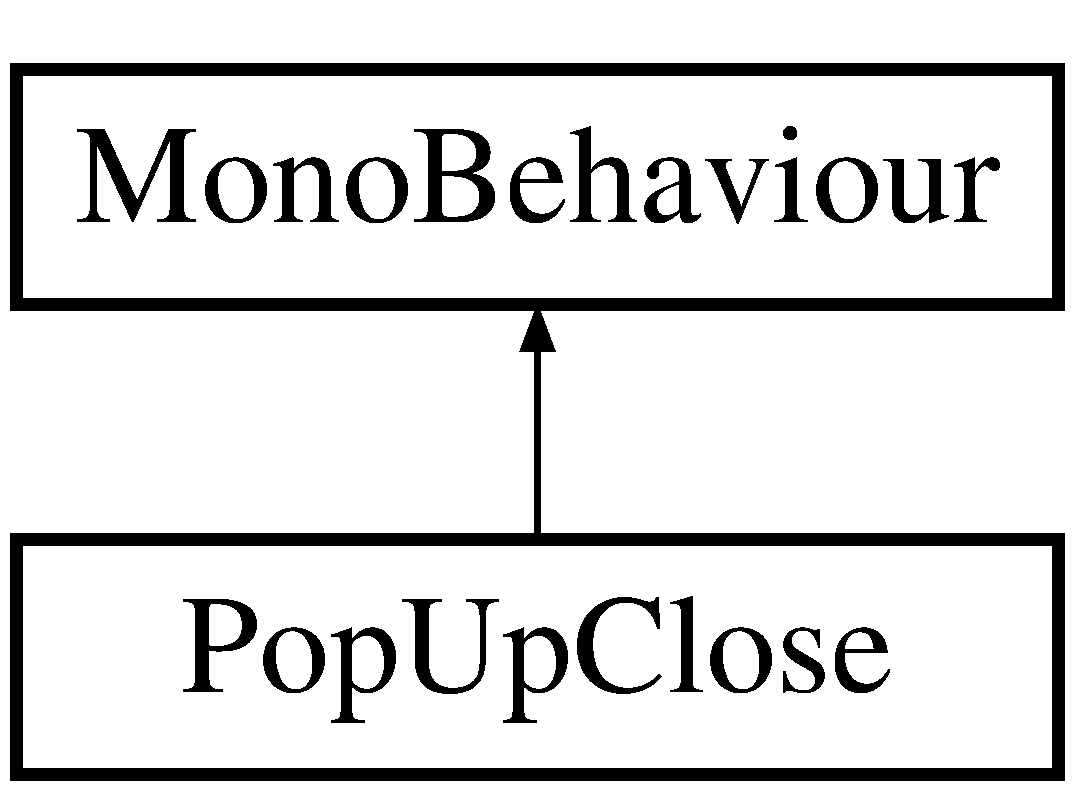
\includegraphics[height=2.000000cm]{class_pop_up_close}
\end{center}
\end{figure}
\subsection*{Fonctions membres publiques}
\begin{DoxyCompactItemize}
\item 
\mbox{\Hypertarget{class_pop_up_close_a49e95ade990c0d89e175aa35c4f1213e}\label{class_pop_up_close_a49e95ade990c0d89e175aa35c4f1213e}} 
void {\bfseries On\+Click} ()
\end{DoxyCompactItemize}


La documentation de cette classe a été générée à partir du fichier suivant \+:\begin{DoxyCompactItemize}
\item 
F\+:/\+Logic\+Gate/\+Logic\+Gate3/\+Unity\+Project/\+Assets/\+Our\+Scripts/Pop\+Up\+Close.\+cs\end{DoxyCompactItemize}

\hypertarget{class_quitter}{}\section{Référence de la classe Quitter}
\label{class_quitter}\index{Quitter@{Quitter}}
Graphe d\textquotesingle{}héritage de Quitter\+:\begin{figure}[H]
\begin{center}
\leavevmode
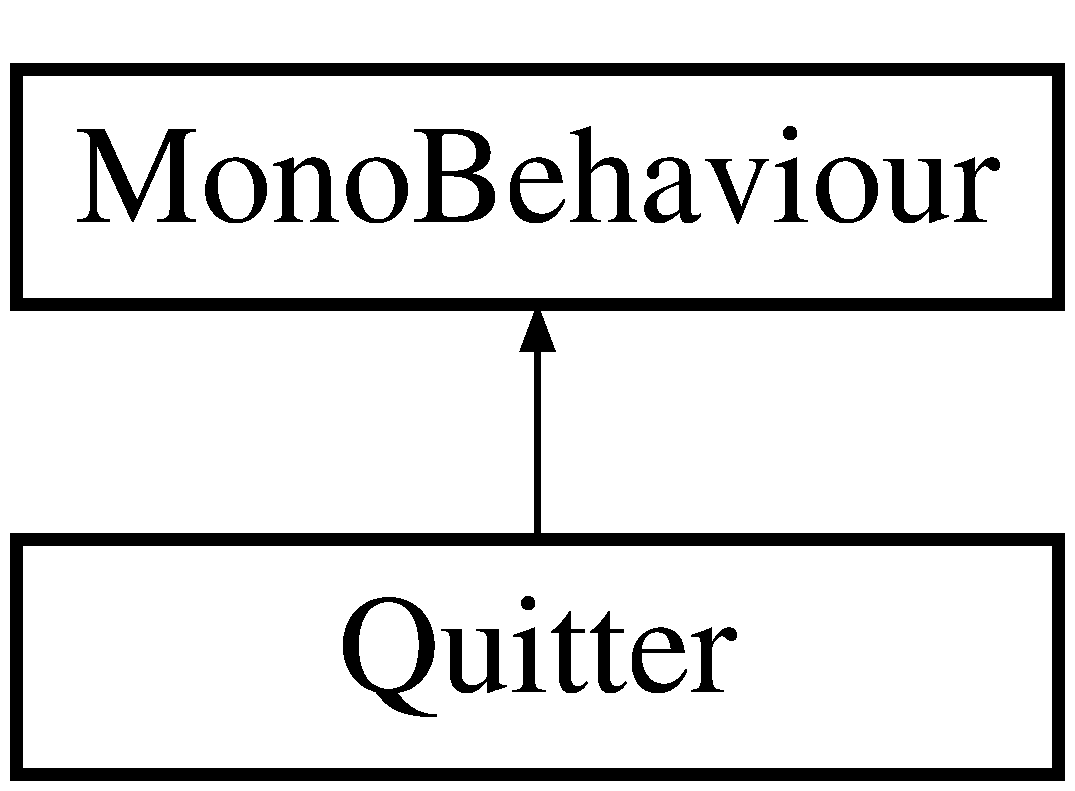
\includegraphics[height=2.000000cm]{class_quitter}
\end{center}
\end{figure}
\subsection*{Fonctions membres publiques}
\begin{DoxyCompactItemize}
\item 
\mbox{\Hypertarget{class_quitter_af10a8e466768e82d4217df76d451268c}\label{class_quitter_af10a8e466768e82d4217df76d451268c}} 
void {\bfseries On\+Click} ()
\end{DoxyCompactItemize}


La documentation de cette classe a été générée à partir du fichier suivant \+:\begin{DoxyCompactItemize}
\item 
F\+:/\+Logic\+Gate/\+Logic\+Gate3/\+Unity\+Project/\+Assets/\+Our\+Scripts/Quitter.\+cs\end{DoxyCompactItemize}

\hypertarget{class_remove_scene}{}\section{Référence de la classe Remove\+Scene}
\label{class_remove_scene}\index{Remove\+Scene@{Remove\+Scene}}
Graphe d\textquotesingle{}héritage de Remove\+Scene\+:\begin{figure}[H]
\begin{center}
\leavevmode
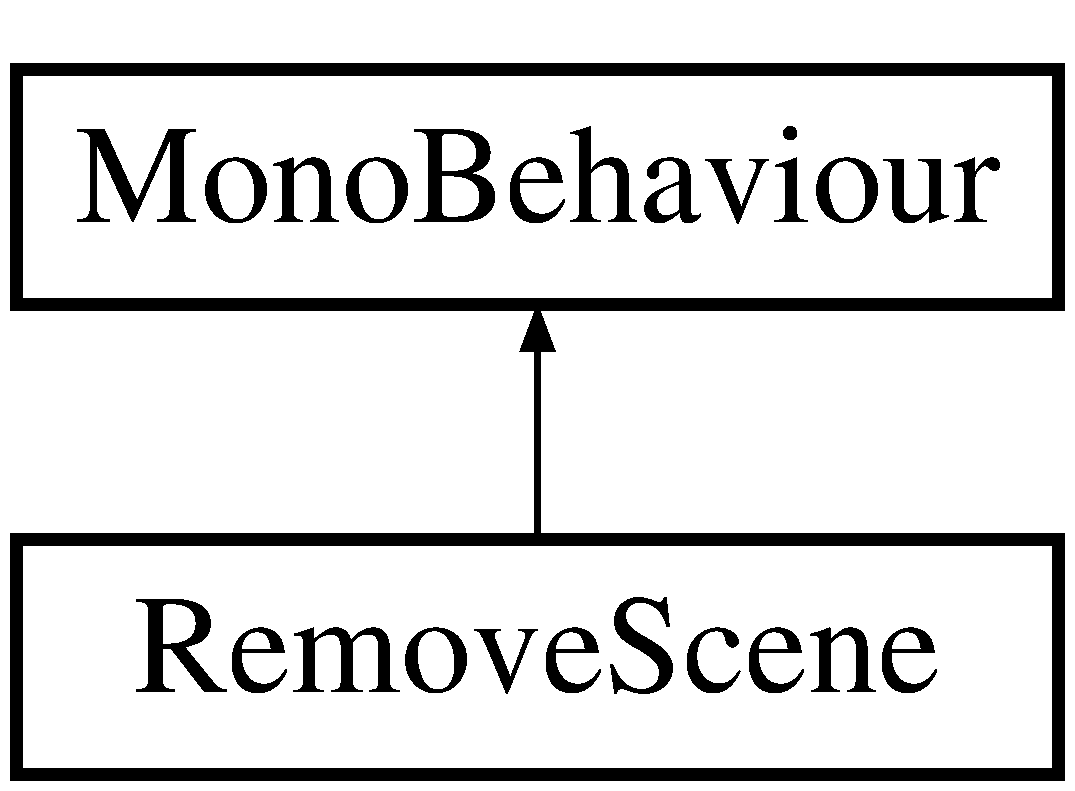
\includegraphics[height=2.000000cm]{class_remove_scene}
\end{center}
\end{figure}
\subsection*{Fonctions membres publiques}
\begin{DoxyCompactItemize}
\item 
\mbox{\Hypertarget{class_remove_scene_af485f2d8ac0b9b72d539a2f2ce7143e6}\label{class_remove_scene_af485f2d8ac0b9b72d539a2f2ce7143e6}} 
void {\bfseries On\+Click} ()
\end{DoxyCompactItemize}
\subsection*{Attributs publics}
\begin{DoxyCompactItemize}
\item 
\mbox{\Hypertarget{class_remove_scene_a0a170dd96a9eebb94e0f9fbaeda7ad51}\label{class_remove_scene_a0a170dd96a9eebb94e0f9fbaeda7ad51}} 
string {\bfseries scene\+To\+Remove}
\end{DoxyCompactItemize}


La documentation de cette classe a été générée à partir du fichier suivant \+:\begin{DoxyCompactItemize}
\item 
F\+:/\+Logic\+Gate/\+Logic\+Gate3/\+Unity\+Project/\+Assets/\+Our\+Scripts/Remove\+Scene.\+cs\end{DoxyCompactItemize}

\hypertarget{class_save_param}{}\section{Référence de la classe Save\+Param}
\label{class_save_param}\index{Save\+Param@{Save\+Param}}
Graphe d\textquotesingle{}héritage de Save\+Param\+:\begin{figure}[H]
\begin{center}
\leavevmode
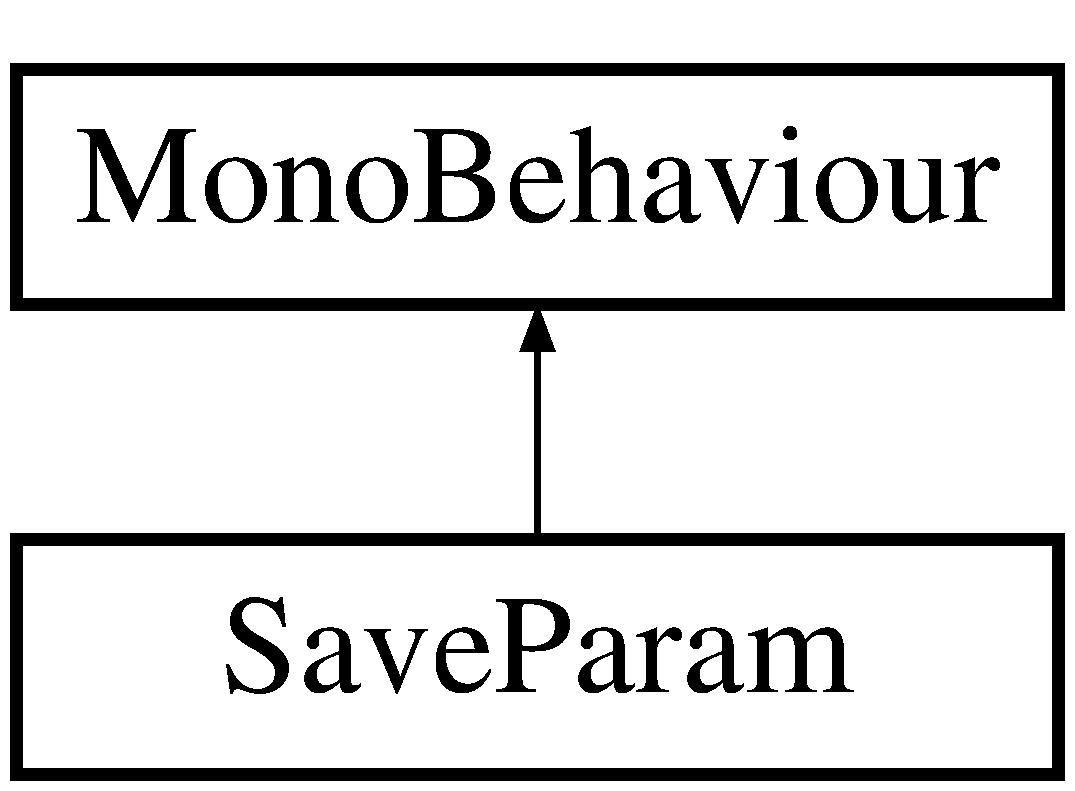
\includegraphics[height=2.000000cm]{class_save_param}
\end{center}
\end{figure}
\subsection*{Fonctions membres publiques}
\begin{DoxyCompactItemize}
\item 
\mbox{\Hypertarget{class_save_param_ae519af3046e225fef106733029d8b774}\label{class_save_param_ae519af3046e225fef106733029d8b774}} 
void {\bfseries save\+\_\+parameters} ()
\end{DoxyCompactItemize}


\subsection{Description détaillée}
Cette classe va permettre de sauvegarder les paramètres dans un fichier binaire à partir de l\textquotesingle{}objet parameter qui les stockent tous. 

La documentation de cette classe a été générée à partir du fichier suivant \+:\begin{DoxyCompactItemize}
\item 
F\+:/\+Logic\+Gate/\+Logic\+Gate3/\+Unity\+Project/\+Assets/\+Our\+Scripts/Save\+Param.\+cs\end{DoxyCompactItemize}

\hypertarget{class_snooze_changer}{}\section{Référence de la classe Snooze\+Changer}
\label{class_snooze_changer}\index{Snooze\+Changer@{Snooze\+Changer}}
Graphe d\textquotesingle{}héritage de Snooze\+Changer\+:\begin{figure}[H]
\begin{center}
\leavevmode
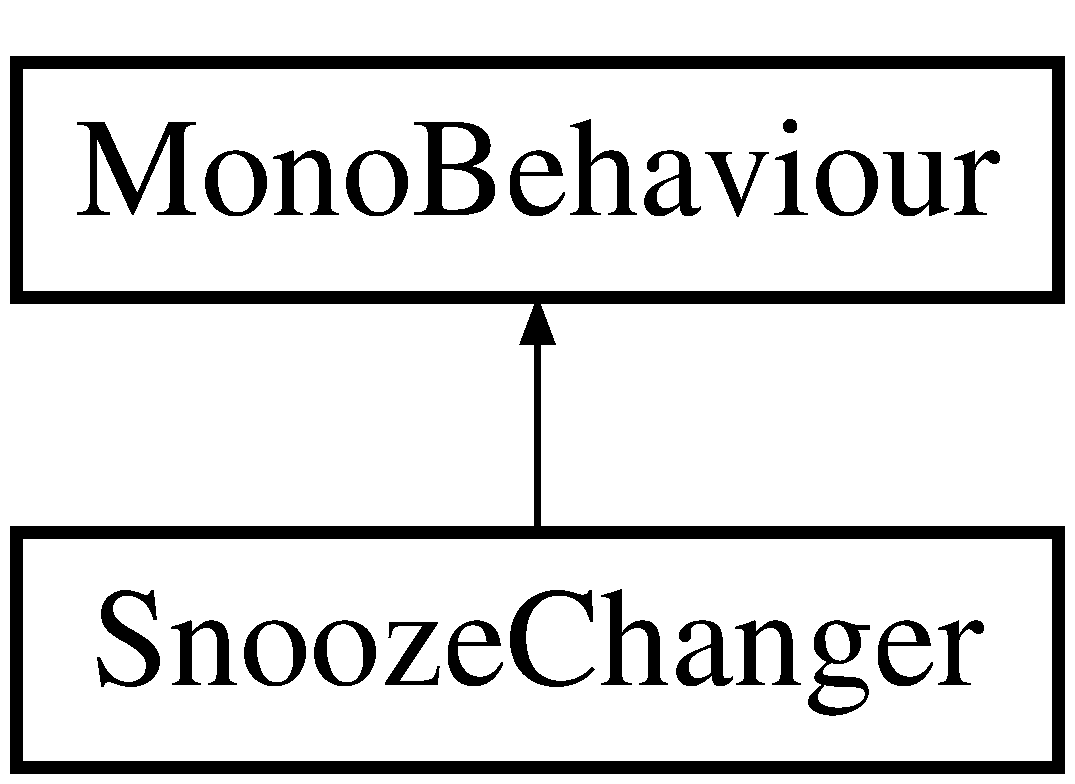
\includegraphics[height=2.000000cm]{class_snooze_changer}
\end{center}
\end{figure}
\subsection*{Fonctions membres publiques}
\begin{DoxyCompactItemize}
\item 
\mbox{\Hypertarget{class_snooze_changer_a24716e3c9890779c20464008605fd603}\label{class_snooze_changer_a24716e3c9890779c20464008605fd603}} 
void {\bfseries Start} ()
\item 
\mbox{\Hypertarget{class_snooze_changer_a9ffaa0bbed0e72bfd0d76be47075e82e}\label{class_snooze_changer_a9ffaa0bbed0e72bfd0d76be47075e82e}} 
void {\bfseries On\+Click} ()
\end{DoxyCompactItemize}


La documentation de cette classe a été générée à partir du fichier suivant \+:\begin{DoxyCompactItemize}
\item 
F\+:/\+Logic\+Gate/\+Logic\+Gate3/\+Unity\+Project/\+Assets/\+Our\+Scripts/Snooze\+Changer.\+cs\end{DoxyCompactItemize}

\hypertarget{class_volume_changer}{}\section{Référence de la classe Volume\+Changer}
\label{class_volume_changer}\index{Volume\+Changer@{Volume\+Changer}}
Graphe d\textquotesingle{}héritage de Volume\+Changer\+:\begin{figure}[H]
\begin{center}
\leavevmode
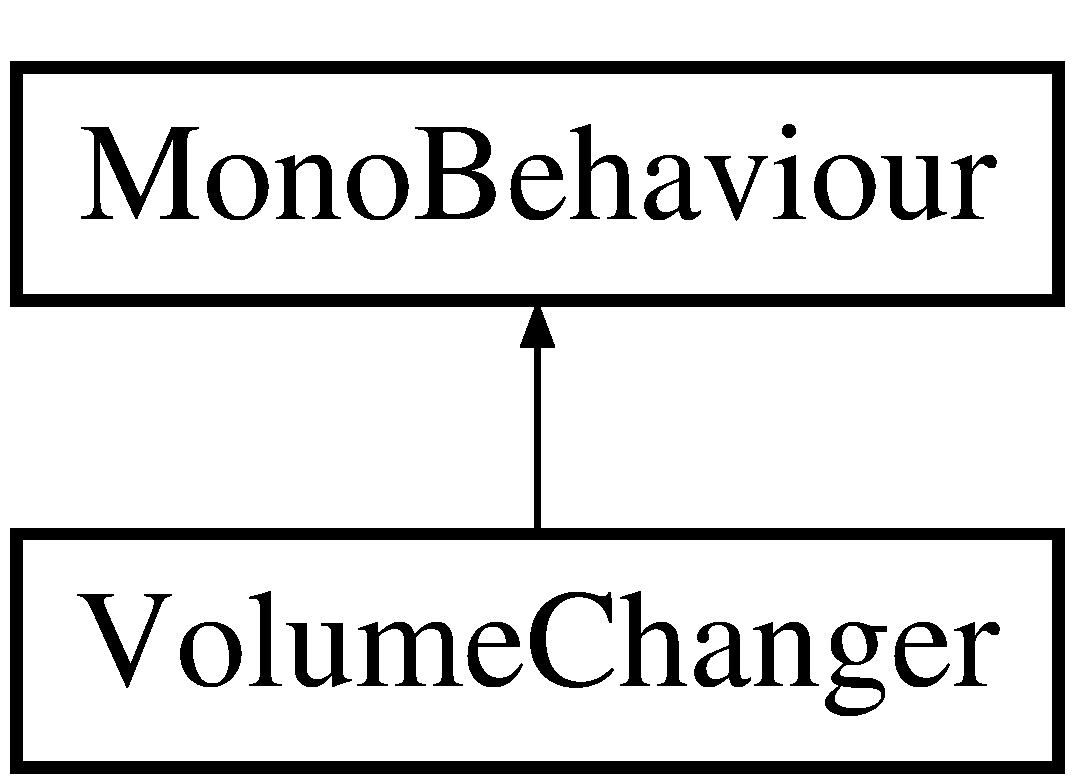
\includegraphics[height=2.000000cm]{class_volume_changer}
\end{center}
\end{figure}
\subsection*{Fonctions membres publiques}
\begin{DoxyCompactItemize}
\item 
\mbox{\Hypertarget{class_volume_changer_a81d7924b367866554520282ca2c238c4}\label{class_volume_changer_a81d7924b367866554520282ca2c238c4}} 
void {\bfseries Start} ()
\item 
\mbox{\Hypertarget{class_volume_changer_a2d5a85ac1481f094c08eb83cbadda336}\label{class_volume_changer_a2d5a85ac1481f094c08eb83cbadda336}} 
void {\bfseries On\+Change} ()
\end{DoxyCompactItemize}


La documentation de cette classe a été générée à partir du fichier suivant \+:\begin{DoxyCompactItemize}
\item 
F\+:/\+Logic\+Gate/\+Logic\+Gate3/\+Unity\+Project/\+Assets/\+Our\+Scripts/Volume\+Changer.\+cs\end{DoxyCompactItemize}

\hypertarget{class_volume_manager}{}\section{Référence de la classe Volume\+Manager}
\label{class_volume_manager}\index{Volume\+Manager@{Volume\+Manager}}
Graphe d\textquotesingle{}héritage de Volume\+Manager\+:\begin{figure}[H]
\begin{center}
\leavevmode
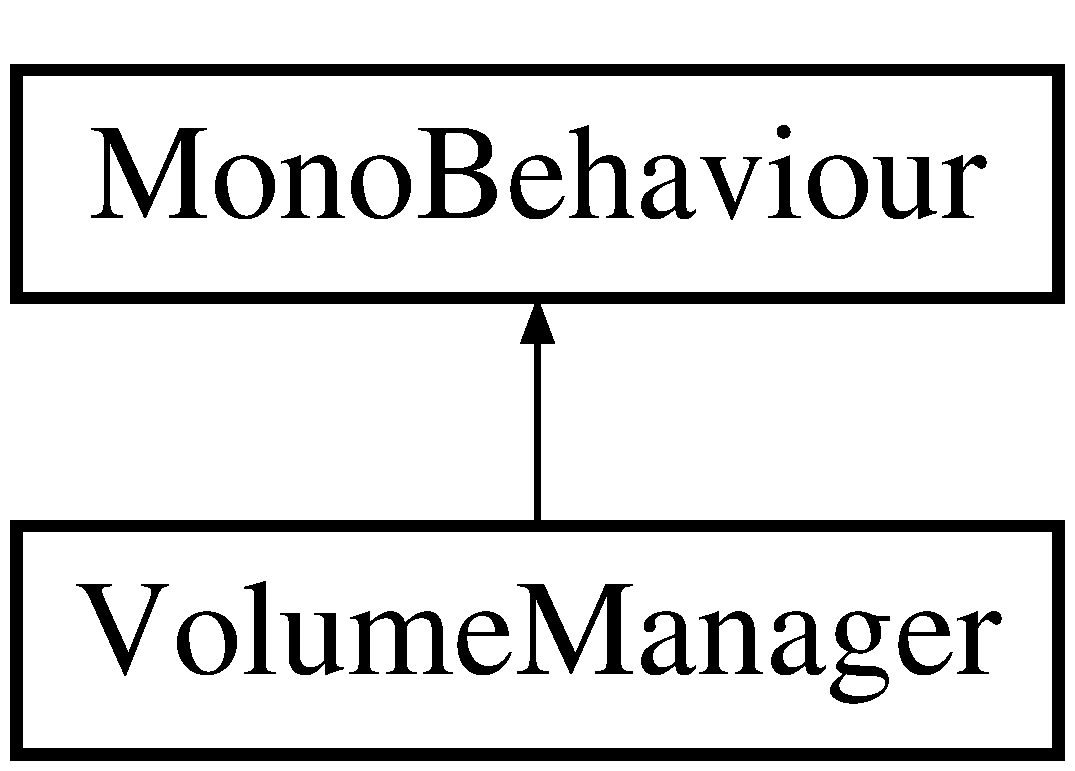
\includegraphics[height=2.000000cm]{class_volume_manager}
\end{center}
\end{figure}


La documentation de cette classe a été générée à partir du fichier suivant \+:\begin{DoxyCompactItemize}
\item 
F\+:/\+Logic\+Gate/\+Logic\+Gate3/\+Unity\+Project/\+Assets/\+Our\+Scripts/Volume\+Manager.\+cs\end{DoxyCompactItemize}

%--- End generated contents ---

% Index
\backmatter
\newpage
\phantomsection
\clearemptydoublepage
\addcontentsline{toc}{chapter}{Index}
\printindex

\end{document}
